\pdfoptionpdfminorversion=4
%DIF LATEXDIFF DIFFERENCE FILE
%DIF DEL ../../manuscript.tex   Tue Jun  7 13:21:04 2022
%DIF ADD ../manuscript.tex      Mon Jun 13 16:26:13 2022

%%%%%%%%%%%%%%%%%%%%%%%%%%%%%%%%%%%%%%%%%%%%%%%%%%%%%%%%%%%%%%%%%%%%%
%% This is a (brief) model paper using the achemso class
%% The document class accepts keyval options, which should include
%% the target journal and optionally the manuscript type.
%%%%%%%%%%%%%%%%%%%%%%%%%%%%%%%%%%%%%%%%%%%%%%%%%%%%%%%%%%%%%%%%%%%%%
\documentclass[journal=jpcbfk,manuscript=article,layout=traditional]{achemso}

%%%%%%%%%%%%%%%%%%%%%%%%%%%%%%%%%%%%%%%%%%%%%%%%%%%%%%%%%%%%%%%%%%%%%
%% Place any additional packages needed here.  Only include packages
%% which are essential, to avoid problems later.
%%%%%%%%%%%%%%%%%%%%%%%%%%%%%%%%%%%%%%%%%%%%%%%%%%%%%%%%%%%%%%%%%%%%%
\usepackage{chemformula} % Formula subscripts using \ch{}
\usepackage[T1]{fontenc} % Use modern font encodings
\usepackage{graphicx}
\usepackage{caption}
\usepackage{amsmath}
\usepackage{mathptmx}
\usepackage[scaled=0.92]{helvet}
%%%%%%%%%%%%%%%%%%%%%%%%%%%%%%%%%%%%%%%%%%%%%%%%%%%%%%%%%%%%%%%%%%%%%
%% If issues arise when submitting your manuscript, you may want to
%% un-comment the next line.  This provides information on the
%% version of every file you have used.
%%%%%%%%%%%%%%%%%%%%%%%%%%%%%%%%%%%%%%%%%%%%%%%%%%%%%%%%%%%%%%%%%%%%%
%%\listfiles

%%%%%%%%%%%%%%%%%%%%%%%%%%%%%%%%%%%%%%%%%%%%%%%%%%%%%%%%%%%%%%%%%%%%%
%% Place any additional macros here.  Please use \newcommand* where
%% possible, and avoid layout-changing macros (which are not used
%% when typesetting).
%%%%%%%%%%%%%%%%%%%%%%%%%%%%%%%%%%%%%%%%%%%%%%%%%%%%%%%%%%%%%%%%%%%%%
\newcommand*\mycommand[1]{\texttt{\emph{#1}}}

%%%%%%%%%%%%%%%%%%%%%%%%%%%%%%%%%%%%%%%%%%%%%%%%%%%%%%%%%%%%%%%%%%%%%
%% Meta-data block
%% ---------------
%% Each author should be given as a separate \author command.
%%
%% Corresponding authors should have an e-mail given after the author
%% name as an \email command. Phone and fax numbers can be given
%% using \phone and \fax, respectively; this information is optional.
%%
%% The affiliation of authors is given after the authors; each
%% \affiliation command applies to all preceding authors not already
%% assigned an affiliation.
%%
%% The affiliation takes an option argument for the short name.  This
%% will typically be something like "University of Somewhere".
%%
%% The \altaffiliation macro should be used for new address, etc.
%% On the other hand, \alsoaffiliation is used on a per author basis
%% when authors are associated with multiple institutions.
%%%%%%%%%%%%%%%%%%%%%%%%%%%%%%%%%%%%%%%%%%%%%%%%%%%%%%%%%%%%%%%%%%%%%
\author{Sree Ganesh Balasubramani}
\affiliation{Department of Chemistry and Biochemistry, University of Arizona, Tucson, Arizona 85721, United States}
\author{Steven D. Schwartz}
\affiliation{Department of Chemistry and Biochemistry, University of Arizona, Tucson, Arizona 85721, United States}
%\author{I. Ken Groupleader}
%\altaffiliation{A shared footnote}
\email{sschwartz@email.arizona.edu}
%\phone{+123 (0)123 4445556}
%\fax{+123 (0)123 4445557}
%\affiliation[Unknown University]
%{Department of Chemistry, Unknown University, Unknown Town}
%\alsoaffiliation[Second University]
%{Department of Chemistry, Second University, Nearby Town}

%%%%%%%%%%%%%%%%%%%%%%%%%%%%%%%%%%%%%%%%%%%%%%%%%%%%%%%%%%%%%%%%%%%%%
%% The document title should be given as usual. Some journals require
%% a running title from the author: this should be supplied as an
%% optional argument to \title.
%%%%%%%%%%%%%%%%%%%%%%%%%%%%%%%%%%%%%%%%%%%%%%%%%%%%%%%%%%%%%%%%%%%%%
\title[]
  {Transition path sampling based calculations of free energies for enzymatic
  reactions: the case of human methionine adenosyl transferase and plasmodium 
  vivax adenosine deaminase}
%%%%%%%%%%%%%%%%%%%%%%%%%%%%%%%%%%%%%%%%%%%%%%%%%%%%%%%%%%%%%%%%%%%%%
%% Some journals require a list of abbreviations or keywords to be
%% supplied. These should be set up here, and will be printed after
%% the title and author information, if needed.
%%%%%%%%%%%%%%%%%%%%%%%%%%%%%%%%%%%%%%%%%%%%%%%%%%%%%%%%%%%%%%%%%%%%%
\abbreviations{TPS,WHAM}
\keywords{American Chemical Society, \LaTeX}

%%%%%%%%%%%%%%%%%%%%%%%%%%%%%%%%%%%%%%%%%%%%%%%%%%%%%%%%%%%%%%%%%%%%%
%% The manuscript does not need to include \maketitle, which is
%% executed automatically.
%%%%%%%%%%%%%%%%%%%%%%%%%%%%%%%%%%%%%%%%%%%%%%%%%%%%%%%%%%%%%%%%%%%%%
%DIF PREAMBLE EXTENSION ADDED BY LATEXDIFF
%DIF UNDERLINE PREAMBLE %DIF PREAMBLE
\RequirePackage[normalem]{ulem} %DIF PREAMBLE
\RequirePackage{color}\definecolor{RED}{rgb}{1,0,0}\definecolor{BLUE}{rgb}{0,0,1} %DIF PREAMBLE
\providecommand{\DIFadd}[1]{{\protect\color{blue}\uwave{#1}}} %DIF PREAMBLE
\providecommand{\DIFdel}[1]{{\protect\color{red}\sout{#1}}}                      %DIF PREAMBLE
%DIF SAFE PREAMBLE %DIF PREAMBLE
\providecommand{\DIFaddbegin}{} %DIF PREAMBLE
\providecommand{\DIFaddend}{} %DIF PREAMBLE
\providecommand{\DIFdelbegin}{} %DIF PREAMBLE
\providecommand{\DIFdelend}{} %DIF PREAMBLE
\providecommand{\DIFmodbegin}{} %DIF PREAMBLE
\providecommand{\DIFmodend}{} %DIF PREAMBLE
%DIF FLOATSAFE PREAMBLE %DIF PREAMBLE
\providecommand{\DIFaddFL}[1]{\DIFadd{#1}} %DIF PREAMBLE
\providecommand{\DIFdelFL}[1]{\DIFdel{#1}} %DIF PREAMBLE
\providecommand{\DIFaddbeginFL}{} %DIF PREAMBLE
\providecommand{\DIFaddendFL}{} %DIF PREAMBLE
\providecommand{\DIFdelbeginFL}{} %DIF PREAMBLE
\providecommand{\DIFdelendFL}{} %DIF PREAMBLE
\newcommand{\DIFscaledelfig}{0.5}
%DIF HIGHLIGHTGRAPHICS PREAMBLE %DIF PREAMBLE
\RequirePackage{settobox} %DIF PREAMBLE
\RequirePackage{letltxmacro} %DIF PREAMBLE
\newsavebox{\DIFdelgraphicsbox} %DIF PREAMBLE
\newlength{\DIFdelgraphicswidth} %DIF PREAMBLE
\newlength{\DIFdelgraphicsheight} %DIF PREAMBLE
% store original definition of \includegraphics %DIF PREAMBLE
\LetLtxMacro{\DIFOincludegraphics}{\includegraphics} %DIF PREAMBLE
\newcommand{\DIFaddincludegraphics}[2][]{{\color{blue}\fbox{\DIFOincludegraphics[#1]{#2}}}} %DIF PREAMBLE
\newcommand{\DIFdelincludegraphics}[2][]{% %DIF PREAMBLE
\sbox{\DIFdelgraphicsbox}{\DIFOincludegraphics[#1]{#2}}% %DIF PREAMBLE
\settoboxwidth{\DIFdelgraphicswidth}{\DIFdelgraphicsbox} %DIF PREAMBLE
\settoboxtotalheight{\DIFdelgraphicsheight}{\DIFdelgraphicsbox} %DIF PREAMBLE
\scalebox{\DIFscaledelfig}{% %DIF PREAMBLE
\parbox[b]{\DIFdelgraphicswidth}{\usebox{\DIFdelgraphicsbox}\\[-\baselineskip] \rule{\DIFdelgraphicswidth}{0em}}\llap{\resizebox{\DIFdelgraphicswidth}{\DIFdelgraphicsheight}{% %DIF PREAMBLE
\setlength{\unitlength}{\DIFdelgraphicswidth}% %DIF PREAMBLE
\begin{picture}(1,1)% %DIF PREAMBLE
\thicklines\linethickness{2pt} %DIF PREAMBLE
{\color[rgb]{1,0,0}\put(0,0){\framebox(1,1){}}}% %DIF PREAMBLE
{\color[rgb]{1,0,0}\put(0,0){\line( 1,1){1}}}% %DIF PREAMBLE
{\color[rgb]{1,0,0}\put(0,1){\line(1,-1){1}}}% %DIF PREAMBLE
\end{picture}% %DIF PREAMBLE
}\hspace*{3pt}}} %DIF PREAMBLE
} %DIF PREAMBLE
\LetLtxMacro{\DIFOaddbegin}{\DIFaddbegin} %DIF PREAMBLE
\LetLtxMacro{\DIFOaddend}{\DIFaddend} %DIF PREAMBLE
\LetLtxMacro{\DIFOdelbegin}{\DIFdelbegin} %DIF PREAMBLE
\LetLtxMacro{\DIFOdelend}{\DIFdelend} %DIF PREAMBLE
\DeclareRobustCommand{\DIFaddbegin}{\DIFOaddbegin \let\includegraphics\DIFaddincludegraphics} %DIF PREAMBLE
\DeclareRobustCommand{\DIFaddend}{\DIFOaddend \let\includegraphics\DIFOincludegraphics} %DIF PREAMBLE
\DeclareRobustCommand{\DIFdelbegin}{\DIFOdelbegin \let\includegraphics\DIFdelincludegraphics} %DIF PREAMBLE
\DeclareRobustCommand{\DIFdelend}{\DIFOaddend \let\includegraphics\DIFOincludegraphics} %DIF PREAMBLE
\LetLtxMacro{\DIFOaddbeginFL}{\DIFaddbeginFL} %DIF PREAMBLE
\LetLtxMacro{\DIFOaddendFL}{\DIFaddendFL} %DIF PREAMBLE
\LetLtxMacro{\DIFOdelbeginFL}{\DIFdelbeginFL} %DIF PREAMBLE
\LetLtxMacro{\DIFOdelendFL}{\DIFdelendFL} %DIF PREAMBLE
\DeclareRobustCommand{\DIFaddbeginFL}{\DIFOaddbeginFL \let\includegraphics\DIFaddincludegraphics} %DIF PREAMBLE
\DeclareRobustCommand{\DIFaddendFL}{\DIFOaddendFL \let\includegraphics\DIFOincludegraphics} %DIF PREAMBLE
\DeclareRobustCommand{\DIFdelbeginFL}{\DIFOdelbeginFL \let\includegraphics\DIFdelincludegraphics} %DIF PREAMBLE
\DeclareRobustCommand{\DIFdelendFL}{\DIFOaddendFL \let\includegraphics\DIFOincludegraphics} %DIF PREAMBLE
%DIF LISTINGS PREAMBLE %DIF PREAMBLE
\RequirePackage{listings} %DIF PREAMBLE
\RequirePackage{color} %DIF PREAMBLE
\lstdefinelanguage{DIFcode}{ %DIF PREAMBLE
%DIF DIFCODE_UNDERLINE %DIF PREAMBLE
  moredelim=[il][\color{red}\sout]{\%DIF\ <\ }, %DIF PREAMBLE
  moredelim=[il][\color{blue}\uwave]{\%DIF\ >\ } %DIF PREAMBLE
} %DIF PREAMBLE
\lstdefinestyle{DIFverbatimstyle}{ %DIF PREAMBLE
	language=DIFcode, %DIF PREAMBLE
	basicstyle=\ttfamily, %DIF PREAMBLE
	columns=fullflexible, %DIF PREAMBLE
	keepspaces=true %DIF PREAMBLE
} %DIF PREAMBLE
\lstnewenvironment{DIFverbatim}{\lstset{style=DIFverbatimstyle}}{} %DIF PREAMBLE
\lstnewenvironment{DIFverbatim*}{\lstset{style=DIFverbatimstyle,showspaces=true}}{} %DIF PREAMBLE
%DIF END PREAMBLE EXTENSION ADDED BY LATEXDIFF

\begin{document}

%%%%%%%%%%%%%%%%%%%%%%%%%%%%%%%%%%%%%%%%%%%%%%%%%%%%%%%%%%%%%%%%%%%%%
%% The "tocentry" environment can be used to create an entry for the
%% graphical table of contents. It is given here as some journals
%% require that it is printed as part of the abstract page. It will
%% be automatically moved as appropriate.
%%%%%%%%%%%%%%%%%%%%%%%%%%%%%%%%%%%%%%%%%%%%%%%%%%%%%%%%%%%%%%%%%%%%%
%\begin{tocentry}

%Some journals require a graphical entry for the Table of Contents.
%This should be laid out ``print ready'' so that the sizing of the
%text is correct.

%Inside the \texttt{tocentry} environment, the font used is Helvetica
%8\,pt, as required by \emph{Journal of the American Chemical
%Society}.

%The surrounding frame is 9\,cm by 3.5\,cm, which is the maximum
%permitted for  \emph{Journal of the American Chemical Society}
%graphical table of content entries. The box will not resize if the
%content is too big: instead it will overflow the edge of the box.

%This box and the associated title will always be printed on a
%separate page at the end of the document.

%\end{tocentry}

%%%%%%%%%%%%%%%%%%%%%%%%%%%%%%%%%%%%%%%%%%%%%%%%%%%%%%%%%%%%%%%%%%%%%
%% The abstract environment will automatically gobble the contents
%% if an abstract is not used by the target journal.
%%%%%%%%%%%%%%%%%%%%%%%%%%%%%%%%%%%%%%%%%%%%%%%%%%%%%%%%%%%%%%%%%%%%%
\begin{abstract}
  Transition path sampling (TPS) is widely used for the
  calculations of reaction rates, transition state structures and reaction 
  coordinates of condensed phase systems. Here we discuss a scheme 
  for the calculation of free energies using the ensemble of TPS reactive 
  trajectories in combination with a window based sampling technique 
  for enzyme catalyzed reactions. We calculate the free energy profiles of 
  the reactions catalyzed by the human methionine S-adenosyltransferase (MAT2A) 
  enzyme and the plasmodium vivax adenosine deaminase ($pv$ADA) enzyme to assess 
  the accuracy of this method. MAT2A catalyzes the formation of S-adenosine-L-methionine
  following a S$_{\text{N}}2$ mechanism and using our method we estimate
  the free energy barrier for this reaction to 
  be $16\;\text{Kcal}\;\text{mol}^{-1}$ which
  is in excellent agreement with the experimentally measured activation 
  energy of $17.27\;\text{Kcal}\;\text{mol}^{-1}$. Furthermore, for the 
  $pv$ADA enzyme catalyzed reaction we estimate a free energy barrier of 
  $23\;\text{Kcal}\;\text{mol}^{-1}$ and the calculated free energy profile is
  similar to that predicted from experimental observations.
  Calculating free energies employing our simple method within TPS 
  provides significant advantages over such methods as umbrella sampling 
  since it is free from any applied external bias, accurate compared to 
  experimental measurements and has a reasonable computational cost.    
\end{abstract}
%%%%%%%%%%%%%%%%%%%%%%%%%%%%%%%%%%%%%%%%%%%%%%%%%%%%%%%%%%%%%%%%%%%%%
%% Start the main part of the manuscript here.
%%%%%%%%%%%%%%%%%%%%%%%%%%%%%%%%%%%%%%%%%%%%%%%%%%%%%%%%%%%%%%%%%%%%%
\section{Introduction}
Molecular dynamics (MD) simulations are increasingly being
used to calculate quantitative estimates of experimentally measurable 
kinetic and thermodynamic parameters of enzyme catalyzed reactions. 
\cite{Karplus02NatStructMolBiol9p646,
Schramm98AnnuRevBiochem67p693,Zhang05AccChemRes38p379,
Schramm11AnnuRevBiochem80p703,Schramm18ChemRev118p11194} 
This has helped in proposing mechanisms and explanations for 
enzyme activity, fast high throughput screening of thousands of inhibitor 
molecules in drug lead discovery, \cite{Jorgensen09AccChemRes42p724,Sliwoski14PharmacolRev66p334} 
directed evolution for designing enzymes with enhanced catalytic 
activities, \DIFdelbegin \DIFdel{\mbox{%DIFAUXCMD
\cite{Thyme09Nature461p1300,Bloom09PNAS106p9995,Schafer19JAmChemSoc141p10431} }\hspace{0pt}%DIFAUXCMD
}\DIFdelend \DIFaddbegin \DIFadd{\mbox{%DIFAUXCMD
\cite{Nunez06JPhysChemA110p463,Thyme09Nature461p1300,
Bloom09PNAS106p9995,Zoi16JAmChemSoc138p3403,Schafer19JAmChemSoc141p10431} }\hspace{0pt}%DIFAUXCMD
}\DIFaddend etc.    
Straightforward MD simulations adequately sample 
the long-lived stable reactant and product states 
but the high energy barrier-crossing events that occur rarely and at long 
time scales are not easily accessible using this method alone.
To access such states at a higher frequency using MD simulations 
several enhanced sampling techniques 
have been developed in the past few decades. These include 
umbrella sampling, \cite{Kastner11WileyInterdiscipRevComputMolSci1p932} 
metadynamics, \cite{Barducci11WileyInterdiscipRevComputMolSci1p826}
steered MD, \cite{Park04JChemPhys120p5946}
milestoning, \cite{Faradjian04JChemPhys120p10880} and transition path sampling 
(TPS). \cite{Pratt86JChemPhys85p5045,Bolhuis02AnnRevPhysChem53p291,
Dellago98JChemPhys108p1964,Bolhuis21AdvTheory4p2000237}

TPS is an attractive method since it samples reactive trajectories
in which the rare barrier-crossing events are guaranteed to occur and
it does not require a priori knowledge of the reaction coordinate which can be 
complex for large biological systems.
TPS is based on Monte Carlo importance sampling in the 
space of trajectories. It uses the shooting and shifting algorithm 
to collect an ensemble of reactive pathways that are real dynamical 
trajectories generated without the application of any bias forces. \cite{dellago02AdvChemPhys123} 
Therefore the TPS ensemble can be used to obtain 
kinetic information such as the rate of the reaction as well as to elucidate 
the transition state, reaction coordinate and the reaction mechanism. 
TPS has been successfully applied to study problems such as enzyme catalysis, 
\DIFdelbegin \DIFdel{\mbox{%DIFAUXCMD
\cite{Antoniou01JPhysChemB105p5553,Hay12NatChem4p161,Schwartz09NatChemBiol5p551} 
}\hspace{0pt}%DIFAUXCMD
}\DIFdelend \DIFaddbegin \DIFadd{\mbox{%DIFAUXCMD
\cite{Basner05JAmChemSoc127p13822,Ramon07JPhysChemB111p5708,Hay12NatChem4p161,Schwartz09NatChemBiol5p551} 
}\hspace{0pt}%DIFAUXCMD
}\DIFaddend and protein folding. \cite{Bolhuis03ProcNatlAcadSci100p12129,Juraszek12ChemPhys396p30}

Calculating equilibrium properties such as the free energy of an enzymatic 
catalysis reaction within TPS is not straightforward. 
The Monte Carlo algorithm used in TPS has an acceptance criterion that 
is only satisfied if the trajectory begins in the reactant basin and ends in 
the product basin or vice versa, hence trajectories that are localized in the 
reactant or product basins, without visiting both are rejected. 
If one defines an order parameter $\zeta$, which separates reactant from 
product basins, then all trajectories, reactive and non-reactive, 
contribute to the probability density distribution function 
($P(\zeta)$) which is the probability of a system at equilibrium to have 
a particular value of the order parameter. \cite{Dellago09AdvCompSimAppp167} 

Frenkel has shown that inclusion of rejected states in a Markov state Monte 
Carlo algorithm can help speed up the convergence of the calculations of 
the order parameter distribution of a two-dimensional
Ising model. \cite{Frenkel04ProcNatAcadSci101p17571}
Inclusion of rejected trajectories within TPS was first discussed by Radhakrishnan 
et al. \cite{Radhakrishnan04JChemPhys121p2436} who developed `BOLAS' which combines 
the shooting and shifting algorithms of TPS with a window based sampling technique 
in the spirit of umbrella sampling to calculate equilibrium free energy 
differences. Peters et al. used a variant of the BOLAS scheme called the 
equilibrium path sampling (EPS) where they use aimless shooting 
combined with window based sampling for free energy calculations. 
\cite{Peters08JAmChemSoc130p17342,Beckham10epsbook} 
More recently Brotzakis et al., \cite{Brotzakis19JChemPhys151p174111}
have developed a re-weighted path ensemble scheme within the standard TPS method 
called virtual interface exchange TPS (VIE-TPS) to calculate the free energy 
landscape. VIE-TPS is shown to produce reasonably accurate free energy profiles for 
chemical reactions that are diffusive in nature whereas it is less accurate otherwise.
Transition interface sampling (TIS) has been used to obtain 
a re-weighted path ensemble which can give access to free energies 
and committor surfaces. \cite{Rogal10JChemPhys17p174109}

Free energy calculations based on the TPS shooting algorithm is 
appealing but rare in the literature. Applications of this 
method to study enzymatic reactions and comparisons of the calculated 
free energies to experimental measurements can shine light on the 
accuracy of this approach compared to the standard methods used for 
free energy calculations.    
In this manuscript we implement and apply the 
algorithm developed by Radhakrishnan et al. \cite{Radhakrishnan04JChemPhys121p2436} 
to calculate the free energies of reactions catalyzed by two systems:
the human MAT2A enzyme and the plasmodium vivax adenosine deaminase 
enzyme. \cite{Luo07JAmChemSoc129p8008,Ho09Biochemistry48p9618}
Human MAT2A catalyzes the formation of S-adenosyl L-methionine (SAM).
SAM is an essential metabolite which is 
distributed to almost all body tissues and fluids, is a universal 
methyl donor and is of fundamental importance to the metabolism of 
compounds such as hormones, neureotransmitters, proteins, 
and nucleic acids. \cite{Friedel89Drugs38p389}
Plasmodium vivax is a parasite that is responsible for the largest number 
of cases of malaria globally. Targeting proteins that are essential to
the metabolism of this bacteria such as the adenosine deaminase enzyme 
is a possible anti-malarial drug development strategy. \cite{Madrid08JBiolChem283p35899} 
These enzymes were chosen not only because of their importance in 
biochemical applications but also because of the availability of experimental 
results with which comparisons can be drawn. This manuscript is organized as 
follows: first we discuss the TPS method and the algorithm that we use 
to calculate the free energies, then we show calculations which apply this 
method on the two enzymatic reactions. Finally we compare our results to experiments
and provide conclusions. 
%------------------------------------------------------------------------------ 
\section{Methods}
%------------------------------------------------------------------------------ 
\subsection{Transition path sampling}
%------------------------------------------------------------------------------ 
Here we briefly describe the equations describing the TPS method for the purpose of
introducing notations as well as for the sake of completeness. 
Consider the molecular dynamics simulation of a molecular system consisting 
of $N$ atoms. Starting from the initial positions and momenta of each atom at time $t_0$,
the time evolution is carried out by finding the position ($\textbf{q}$) and 
momenta ($\textbf{p}$) of each atom at regular intervals of time $t_i = t_0 + i\Delta t$  
($i = 0,1,2,\ldots$). At each of the time slices, the positions and 
momenta can be collectively represented as
the set $z = \{\textbf{q},\textbf{p}\}$. If the MD simulation is 
run for a total 
time of $\mathcal{T}$ the number of time slices is given by 
$L = \mathcal{T}/\Delta t +1$ and for this sequence of 
times the state of the system can be represented as 
\begin{equation}
z(\mathcal{T}) = \{z_0, z_{\Delta t}, z_{2\Delta t},\ldots,z_{\mathcal{T}}\}
\end{equation}
The probability to obtain a particular sequence of states is determined by the initial 
conditions and the type of dynamics used for the time evolution. If the time evolution is 
Markovian, the probability to go from $z_{i\Delta t}$ to $z_{(i+1)\Delta t}$ depends only 
on $z_{i\Delta t}$ and not on conditions before the time $i\Delta t$ the total path probability can 
be expressed as the product of individual probabilities $p(i\rightarrow j)$ as 
\begin{equation}
\mathcal{P}[z(\mathcal{T})] = \rho(z_0)\Pi_{i=0}^{\mathcal{T}/\Delta t-1} p(z_{i\Delta t}\rightarrow z_{(i+1)\Delta t}),
\end{equation}
where $\rho(z_0)$ is the equilibrium distribution of the initial conditions and for a canonical ensemble this can be 
expressed as 
\begin{equation}
\rho(z_0) = \exp(-\beta H(z_0))/Z
\end{equation}
where 
\begin{equation}
Z = \int dz \exp(-\beta H(z)) 
\end{equation}
is the canonical partition function. 

Within the transition path sampling, the trajectories of interest start in the reactant region of the 
phase space ($\mathcal{A}$) and end in the product region ($\mathcal{B}$). Such reactive trajectories have 
a restricted probability distribution function given by
\begin{equation}
\mathcal{P}_{\mathcal{AB}}[z_{\mathcal{T}}] = h_{\mathcal{A}}(z_0)\mathcal{P}[z(\mathcal{T})]
h_{\mathcal{B}}(z_{\mathcal{T}})/Z_{\mathcal{AB}}(\mathcal{T})\label{eqn:tpsensem}
\end{equation}
where 
\[
    h_{\mathcal{A}/\mathcal{B}}(z)= 
\begin{cases}
    1, & \text{if } z\in \mathcal{A}/\mathcal{B}\\
    0,              & \text{otherwise}
\end{cases}
\]
and $Z_{\mathcal{AB}}(\mathcal{T})$ is the normalization factor for this 
probability distribution function.
The set of all reactive trajectories characterized by the probability 
distribution function given by Eq. \ref{eqn:tpsensem} is the 
transition path ensemble. 

\subsection{Equilibrium distribution of order parameters}
The free energy of a molecular system as a function of the order parameter $\zeta$ 
is defined as 
\begin{equation}
\text{A}(\zeta) = -k_{\text{B}}T\text{ln}(P(\zeta)) + C, \label{eqn:fenergy}
\end{equation}
where $P(\zeta)$ is the probability distribution function of the reaction coordinate
$\zeta$, $C$ is an arbitrary constant, $k_{\text{B}}$ is the Boltzmann constant
and $T$ is the temperature. At equilibrium the probability distribution of the 
reaction coordinate can be obtained from the distribution function for the phase 
space $\rho(\textbf{q})$ as
\begin{equation}
P(\zeta) = \int d\textbf{V} \rho(\textbf{q})\delta\left[\zeta-\tilde{\zeta}(\textbf{q})\right].
\end{equation}
The integration is over the entire phase space. In practice, the calculation of this distribution function
often proceeds using histogram based methods where the reaction coordinate is 
divided into bins and the frequency of the occurrence of the reaction coordinate 
within a particular window during the course of MD simulation is used to calculate 
the probability distribution function. Since some values of the reaction coordinates 
particularly close to the transition state are 
rarely sampled in a conventional MD simulations, enhanced sampling techniques such as the umbrella sampling
are necessary to sample the low probability regions. TPS is designed to sample these regions in phase space 
without the application of any external bias, but the trajectories 
sampled with TPS are only reactive and hence
they are not distributed according to the equilibrium distribution function. 
The restriction that the pathways start from the reactant state and end in the 
product state can be relaxed to obtain an ensemble of trajectories that will 
be distributed according to the equilibrium distribution. 
%------------------------------------------------------------------------------ 
\subsection{Algorithm for free energy calculations}\label{ssec:algorithm}
%------------------------------------------------------------------------------ 
We follow the steps proposed by Radhakrishnan et al. \cite{Radhakrishnan04JChemPhys121p2436} 
to sample TPS trajectories within windows of the order parameter. 
\begin{itemize}
\item An appropriate order parameter is chosen for the reaction of interest 
that can distinguish the reactant and product states sufficiently well and the TPS ensemble is harvested 
which consists only of reactive trajectories.
\item The order parameter is divided into windows $\{\zeta_i\}$ and within each window,
$\zeta_{i}^{min} < \zeta < \zeta_{i}^{max}$ is to be sampled.
\item Choose a reactive trajectory $\tilde{z}(\mathcal{T})$ from the TPS ensemble as 
a guiding trajectory for the window sampling. Pick a time slice from this trajectory 
$\tilde{z}_{j\Delta t}$ such that the order parameter calculated for this time slice
$\tilde{\zeta}$ satisfies $\zeta_{i}^{min} < \tilde{\zeta} < \zeta_{i}^{max}$.
\item Using the shooting and shifting algorithm familiar from TPS simulations, \cite{dellago02AdvChemPhys123}
harvest dynamics trajectories starting from the time slice $\tilde{z}_{j\Delta t}$ of the trajectory 
$\tilde{z}(\mathcal{T})$ and accept the new trajectory if for any time slice the calculated 
order parameter $\hat{\zeta}$ satisfies $\zeta_{i}^{min} < \hat{\zeta} < \zeta_{i}^{max}$.
\item Calculate the probability distribution ($P_i(\zeta)$) within the window $\zeta_{i}^{min} 
< \zeta < \zeta_{i}^{max}$ by constructing histograms obtained from the ensemble of 
accepted trajectories for the window referenced by the index $i$. 
\item Calculate the free energies for each of the windows according to Eq. \ref{eqn:fenergy}
and combine them such that the function $\text{A}(\zeta)$ is continuous 
by adjusting the constants $C$. 
\end{itemize}
%------------------------------------------------------------------------------ 
\section{Computational details}
%------------------------------------------------------------------------------ 
\subsection{System preparation}
%------------------------------------------------------------------------------
We used the crystal structure of the human MAT2A enzyme 
bound to methylthioadenosine and di-imido triphosphate (PNPNP)
(protein data bank ID: 7L1A) reported by Niland 
et al. \cite{Niland21Biochem60p791,Ghosh21JAmChemSoc143p18325} and the crystal 
structure of \textit{pv}ADA in complex with MT-coformycin (protein data bank ID: 3EWC) 
reported by Ho et al. \cite{Ho09Biochemistry48p9618} as the starting points of our two 
simulations. For calculations involving the MAT2A enzyme the substrates were modified to 
L-methionine and adenosyl triphosphate (ATP) whereas for calculations with the \textit{pv}ADA
enzyme the substrates were modified to $2^{'}-$deoxyadenosine and hydroxide ion. 
We solvated both the systems using TIP3P water molecules \cite{Jorgensen83JChemPhys79p926}
in a nanodroplet sphere whose volume was fixed at $15$ {\AA}
away from the protein's surface and the total charge was neutralized 
using potassium ions. 

MD simulations within classical and hybrid quantum mechanics/molecular mechanics 
(QMMM) approximations were carried out using the CHARMM program 
package. \cite{Brooks83JComputChem4p187} 
For the MM calculations the CHARMM36 force field \cite{Brooks09JComputChem30p1545} 
was used and for the QM calculations the approximate PM3 semiempirical 
method \cite{Repasky02JComputChem23p1601} was used. 
For the hybrid QMMM simulations, the MAT2A system was partitioned into a QM
region consisting of the ATP and MET molecules along with three Mg$^{2+}$ ions 
and the MM region consists of the rest of the molecules. 
For the $pv$ADA system the QM region consisted of 
the adenosine molecule, an hydroxide anion, Zn$^{2+}$ ion and 
a portion of the Glu229 residue which was partitioned within the generalized 
hybrid orbital (GHO) scheme. \cite{Gao98JPhysChemA102p4714}  

The energies of both the systems were minimized using 50 steps of the 
steepest descent method, followed by 2000 steps of the
adopted basis Newton-Raphson method where only classical molecular mechanics 
was used for the dynamics. 
The minimized systems were
heated slowly to 300 K for 35 ps beginning with harmonic
constraints on all atoms except on the H atoms and the TIP3P 
water molecules with gradual reduction of the restraint forces. 
15 ps of equilibration was carried out starting with harmonic 
restraint forces followed by 20 ps of constraint free 
equilibration to prepare the systems for TPS simulations. 
During the heating and equilibration steps, bonds that contain 
hydrogen atoms in the MM region were restrained to their equilibrium values 
using the SHAKE procedure. \cite{Ryckaert77JComputPhys23p327} 
%------------------------------------------------------------------------------ 
\subsection{Transition path sampling}
%------------------------------------------------------------------------------
TPS simulations require the definition of unique reactant and product states
to collect reactive trajectories based on the Monte Carlo algorithm. Here we 
discuss the details of the reactions involving the MAT2A and the $pv$ADA enzymes 
to identify and define the order parameters characterizing the reactant and product basins.  

The reaction catalyzed by the human MAT2A enzyme is
between adenosyl $5'$-triphosphate (ATP) and L-methionine (MET) molecules 
resulting in the formation of S-adenosyl-L-methionine (SAM) which is 
depicted in Fig. \ref{fig:mat2a-reaction}. This reaction follows a S$_{\text{N}}2$ 
mechanism and was experimentally characterized by 
Firestone et al. \cite{Firestone17JAmChemSoc139p13754}. The key bond 
parameters for this reaction consists of the distance between the
nucleophilic sulfur atom of MET and the $5'-C$ atom of the ATP (denoted as d$_{\mathrm{SC}}$), 
and the distance between oxygen atom of the phosphate group and the $5'-C$ 
atom of ATP (d$_{\mathrm{OC}}$). For the TPS calculations we define the 
reactant state to have d$_{\mathrm{OC}}$ to be less than 1.7 {\AA} and the product 
state to have the d$_{\mathrm{SC}}$ less than 2.0 {\AA}. 

\begin{figure}

\includegraphics[width=\columnwidth]{figures/mat2a-reaction.png}
\caption{The reaction catalyzed by the human MAT2A enzyme between ATP and L-methionine resulting in the 
formation of S-adenosyl L-methionine and triphosphate leaving group.}
\label{fig:mat2a-reaction}
\end{figure}

$pv$ADA catalyzes the reaction between adenosine and OH$^{-}$ anion
resulting in the formation of inosine and ammonia as shown in
Fig. \ref{fig:ada-reaction}.
The nucleophilic O atom of the OH$^{-}$ anion
attacks the electrophilic C6 atom of the adenosyl ring leading to the 
formation of a Meisenheimer complex like structure while the N1 atom 
on the adenosyl moiety gets protonated by the Glu229 residue of $pv$ADA. 
The key bond parameters are the distance between the approaching hydroxyl 
oxygen and the C6 atom (denoted as d$_{\text{OC}}$) and the 
dissociating C6$-$N6 (d$_{\text{NC}}$) bond distance. For the TPS simulations 
we define the reactant state to have d$_{\text{NC}}$ being less than $1.8$ {\AA} 
and the product state to have the d$_{\text{OC}}$ less than $1.8$ {\AA}.

\begin{figure}

\includegraphics[width=\columnwidth]{figures/ada-reaction.png}
\caption{The reaction catalyzed by the $pv$ADA enzyme between adenosine and hydroxide ion
resulting in the formation of inosine and ammonia.}
\label{fig:ada-reaction}
\end{figure}

A biased initial reactive trajectory is obtained by using harmonic restraint forces 
for both the MAT2A and $pv$ADA systems.
\DIFaddbegin \DIFadd{For the MAT2A system harmonic constraint with a force constant of 35 kcal mol$^{-1}$ }{\DIFadd{\AA}}\DIFadd{$^{-2}$
was used for the bond breaking C5-O5 distance and the bond forming SD-C5 distance,
and dynamics was run for $500\;fs$ starting with the reactant state and ending up in the product state.   
For the $pv$ADA system harmonic constraints with a force constant of 40 kcal mol$^{-1}$}{\DIFadd{\AA}}\DIFadd{$^{-2}$ 
was used for the bond breaking (C6-N6) and bond forming (O1-C6) distances, and for the proton 
transfer distances between the OE2 atom on the GLU229 residue to the N1 atom on 
the adenosyl moeity and the dynamics was propagated for $500\;fs$ going from the reactant to 
the product state. }\DIFaddend Using the biased trajectory as the starting point and after removing the restraint 
forces, the shooting algorithm \cite{dellago02AdvChemPhys123} was used to generate
new trajectories. The shooting algorithm begins with the choice of a 
random time slice from the biased initial reactive trajectory and perturbs 
the momenta of all the atoms in the system. Then the dynamics is propagated for 
250 steps forwards and backwards using $1\;fs$ time steps
resulting in a trajectory with a time period of $0.5\;ps$.
\DIFaddbegin \DIFadd{The trajectories were propagated for a longer $1\;ps$ time period 
to make sure that the chemical reaction occurs within $0.5\;ps$. 
}\DIFaddend A total of 150 reactive trajectories were generated for both the MAT2A and $pv$ADA
systems. \DIFaddbegin \DIFadd{The percentage of TPS trajectories that were accepted were 24$\%$ and 
19$\%$ for the MAT2A and $pv$ADA systems, respectively.
For optimal sampling with a good balance between the number of 
accepted reactive trajectories and decorrelation from the initial constrained
trajectory as well from one another, the acceptance percentage 
is typically $\sim$ 40. \mbox{%DIFAUXCMD
\cite{dellago02AdvChemPhys123}  
}\hspace{0pt}%DIFAUXCMD
For complex systems such as enzymes we find that the lower the acceptance 
percentage the quicker is the decorrelation. 
%DIF > While a 40$\%$ acceptance has been found to provide the best compromise between the
%DIF > number of accepted trajectories and decorrelation of the
%DIF > trajectories from one another, 
%DIF > we find that a lower acceptance
%DIF > ratio provides quicker decorrelation from the initial constrained
%DIF > trajectory, especially in more complex systems such as enzymes.
}\DIFaddend %------------------------------------------------------------------------------ 
\subsection{Free energy calculations}
%------------------------------------------------------------------------------ 
We follow the algorithm discussed previously to calculate the free energy
profile for the two enzymatic reactions using the TPS reactive trajectories. 
The order parameter for the MAT2A system 
is defined to be d$_{\text{OC}}-$d$_{\text{SC}}$ and that for the $pv$ADA is defined as 
d$_{\text{NC}}-$d$_{\text{OC}}$. For the MAT2A system, configurations are sampled
for order parameter values within the range $[-2.0,2.0]$ and this range is divided 
into 14 overlapping windows ($0.09$ {\AA} between neighboring windows). 
Configurations are sampled for the $pv$ADA system for order parameter values 
within the interval $[-3.0, 3.0]$ {\AA} which is divided into 20 overlapping 
windows ($0.09$ {\AA} between neighboring windows). A reactive 
trajectory from the TPS ensemble is chosen to guide the sampling 
within each of the windows in the same spirit as a steered MD trajectory 
is used to guide the window based umbrella sampling simulations (though in this case,
of course, this is an unbiased dynamically exact reactive trajectory). 
To sample in a particular window $\zeta_i$, a frame from this reactive 
trajectory is chosen such that the value of its 
order parameter ($\zeta$) falls within 
$\zeta_{i}^{min} < \zeta < \zeta_{i}^{max}$. Using the shooting algorithm
the momenta of all the atoms in the system are perturbed 
and dynamics is run for 10 steps forwards and backwards with a 
$1\;fs$ time step to obtain a trajectory with a time period of $20\;fs$.
Longer trajectories in our experience end up sampling outside the window 
more often and hence we make use of very short trajectories in this study.     
Within each window 3000 TPS trajectories are collected. The 
probability distribution function for the order parameter within window $w$ 
is then calculated as normalized histograms which represent the populations 
of the configurations within the window at equilibrium. 
Finally we calculate the free energy profile in a similar fashion to the WHAM 
procedure \cite{Kumar92JComputChem13p1011} which is generally used to obtain the 
potential of mean force from umbrella sampling calculations. 
%------------------------------------------------------------------------------ 
\section{Results and discussion}
%------------------------------------------------------------------------------ 
\subsection{Human MAT2A}
The equilibrated structure of the MAT2A enzyme in complex with 
ATP, MET and two Mg$^{2+}$ ions is shown in Fig. \ref{fig:mat2a-equil}.
\begin{figure}[ht!]
\centering
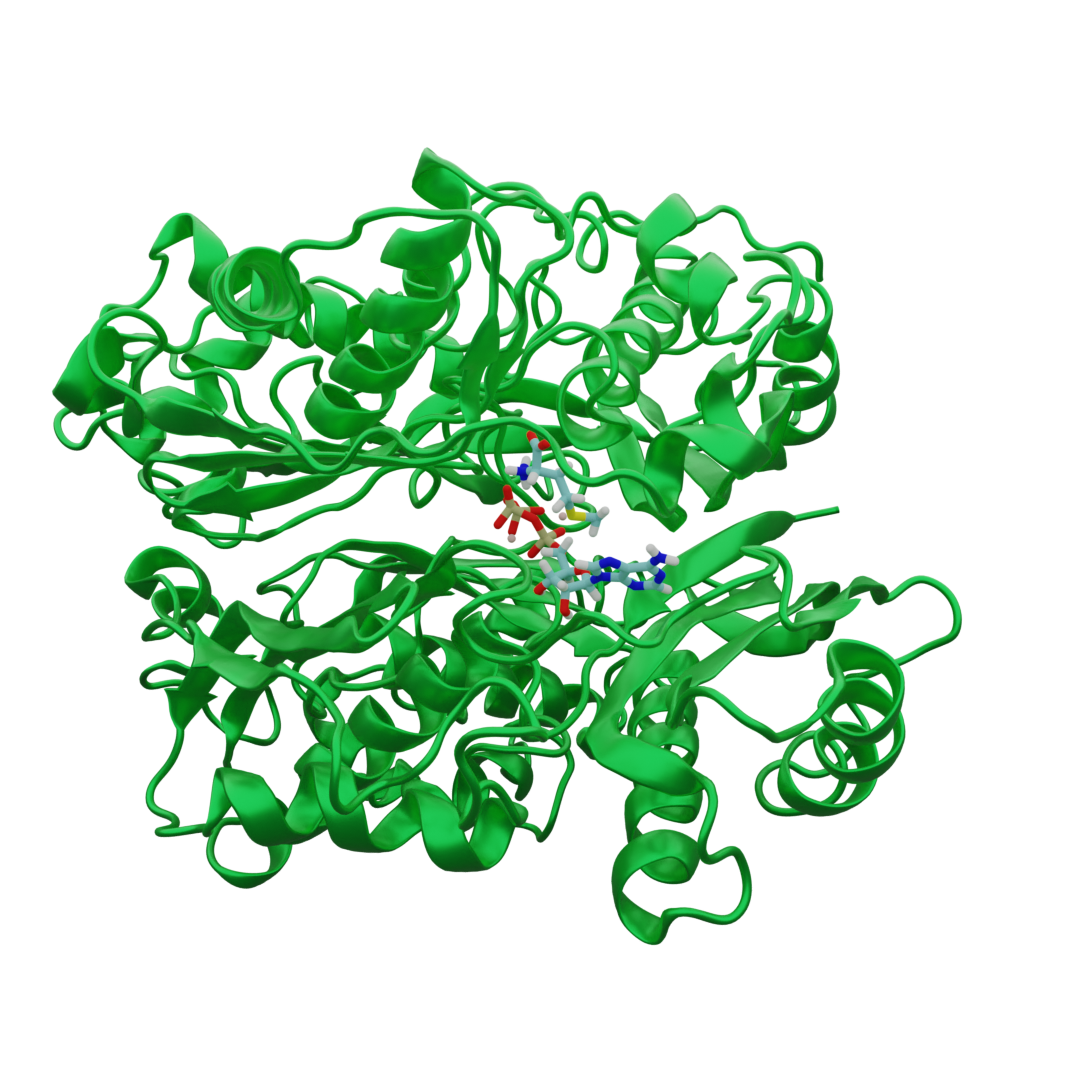
\includegraphics[scale=0.2]{figures/mat2a-equil.png}
\caption{Equilibrated structure of the MAT2A enzyme in complex with ATP and 
MET along with 2 Mg$^{2+}$ ions.}
\label{fig:mat2a-equil}
\end{figure}
The variation of the key distance parameters of the reaction calculated for 
a reactive trajectory from the TPS ensemble are shown in Fig. \ref{fig:mat2a-reactive-traj}.
\begin{figure}
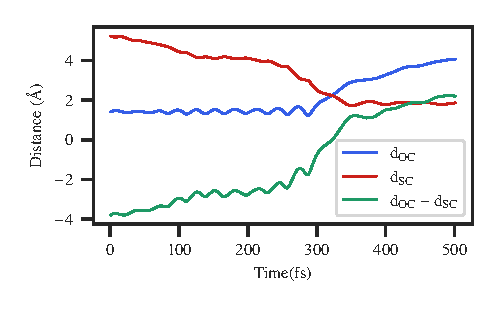
\includegraphics[scale=1.0]{figures/mat2a-diff167.pdf}
\caption{Bond breaking ($\mathrm{d}_{\mathrm{OC}}$), bond forming 
($\mathrm{d}_{\mathrm{SC}}$) distances for a typical 
reactive trajectory for the reaction catalyzed by the MAT2A enzyme.}
\label{fig:mat2a-reactive-traj}
\end{figure}
Committor analysis and committor distribution analysis are used to deduce 
the transition states and the reaction coordinates, respectively. 
Committor analysis is carried out for a reactive trajectory 
from the TPS ensemble by choosing a time slice randomly from the trajectory, assigning
momenta picked at random from the Boltzmann distribution for all the atoms, and running 
dynamics for $250\;fs$. The commitment probability of a time slice is calculated by 
repeating this procedure \DIFdelbegin \DIFdel{many times }\DIFdelend \DIFaddbegin \DIFadd{at least 50 times for each time slice }\DIFaddend and finding the fraction of trajectories that go 
to the reactant, product or neither. The transition state for the reaction is defined as 
the structure from the time slice that has equal probability to commit to the reactant 
and the product state. Repeating this process for several trajectories from the TPS
ensemble results in a collection of transition states called the separatrix. \DIFaddbegin \DIFadd{We calculated 
11 transition state structures for the MAT2A and the }\textit{\DIFadd{pv}}\DIFadd{ADA enzymes and details 
regarding them are reported in the supporting information. 
}\DIFaddend \begin{figure}[ht!]
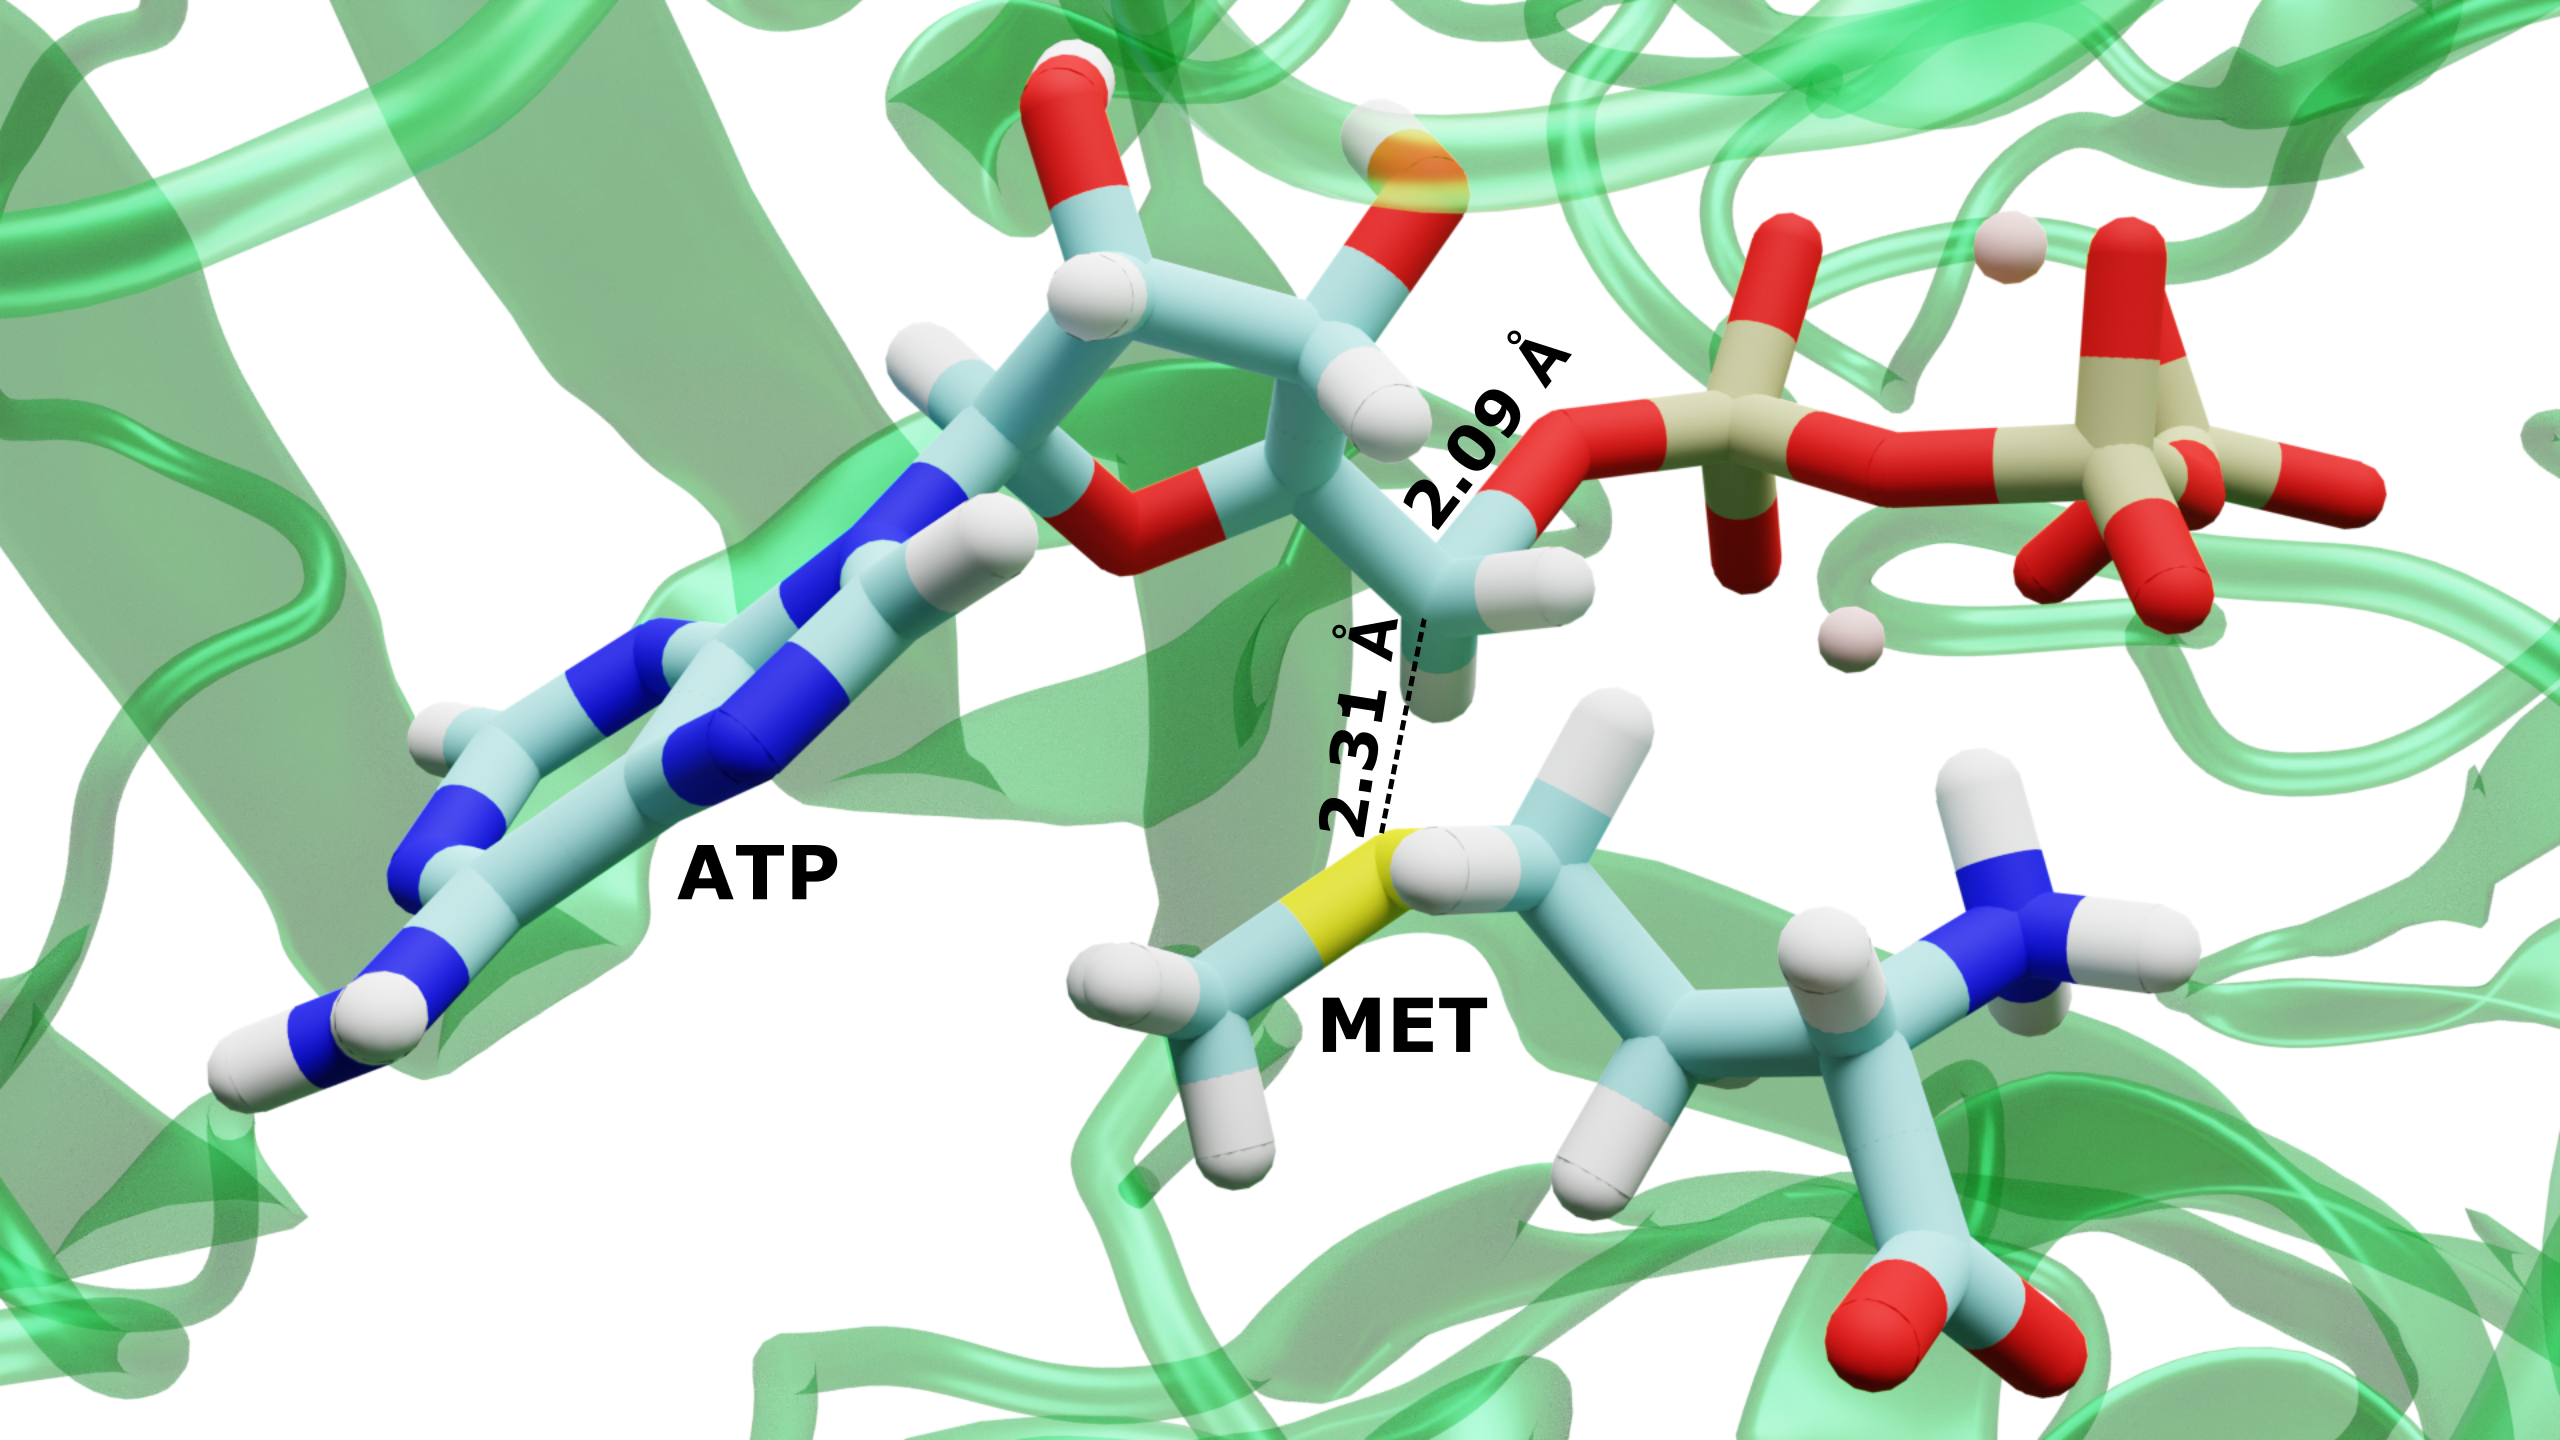
\includegraphics[scale=0.12]{figures/mat2a-trans-labelled.png}
\caption{Transition state structure of the reaction catalyzed by the human MAT2A enzyme.
The bond parameters d$_{\text{SC}}$ and d$_{\text{OC}}$ are $2.31$ {\AA} and $2.09$ {\AA}, 
respectively.}
\label{fig:mat2a-trans-struct}
\end{figure}
The transition state resembles a S$_{\text{N}}2$ structure with the 
d$_{\text{SC}}$ and d$_{\text{OC}}$ distances being $2.31$ {\AA} and $2.09$ {\AA}, respectively.
Experimentally the transition state structures of enzymatic reactions
can be elucidated using kinetic isotope effects (KIE). \cite{Schramm99MetEnzym308p301}
Firestone et al. \cite{Firestone17JAmChemSoc139p13754} used a combination of experimental 
KIE measurements using the whole protein system and computational density functional 
theory (DFT) based gas phase simulations of representative molecules to elucidate the 
transition state structure for this reaction. From their findings they report 
d$_{\text{SC}}$ and d$_{\text{OC}}$ distances of $2.03$ {\AA} and $2.32$ {\AA}, 
respectively and our calculated values are in close agreement to this result. 

The reaction coordinate might contain not just the atoms from the molecules that 
are directly involved in the reaction but also residues from side chains that can 
promote the reaction. \cite{Schramm18Biochem57p3299} Taking this into account the 
committor distribution analysis
begins by constraining the residues and molecules that are hypothesized to be part of the 
reaction coordinate and using this constrained system as the starting point 
trajectories are launched assigning momenta at random from the Boltzmann distribution at 
$300\;\text{K}$ to all the atoms in the system. 
First we constrained just the QM region in our committor distribution analysis 
which consists of ATP and MET molecules along with two Mg$^{2+}$ ions and the 
resulting distribution as shown in Fig. \ref{fig:mat2a-comm-dist} is not peaked 
at 0.5 which is expected for the reaction coordinate. 
Next we constrained the residues Gln113, Ser114, Arg249 and Arg264 along with the 
QM region and obtain a distribution that is peaked at 0.5 and hence we 
conclude that the reaction coordinate consists of these residues as well. 
\begin{figure*}[ht!]
\centering
\begin{minipage}[b]{0.45\linewidth}
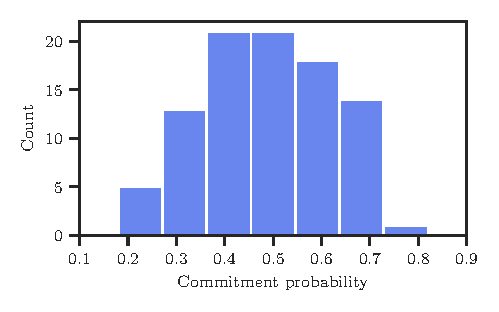
\includegraphics[width=\textwidth]{figures/comm-60-mat2a-nocons.pdf}
\label{fig:minipage1}
\end{minipage}
\quad
\begin{minipage}[b]{0.45\linewidth}
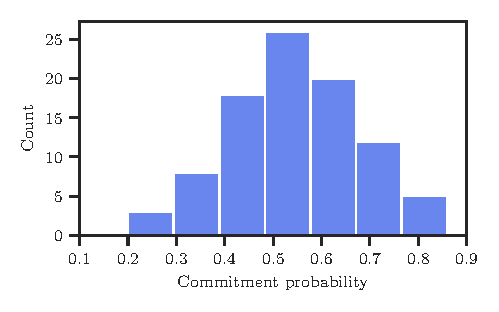
\includegraphics[width=\textwidth]{figures/comm-60-mat2a.pdf}
\label{fig:minipage2}
\end{minipage}
\caption{Committor distribution analysis for obtaining the reaction coordinate of the 
MAT2A catalyzed reaction. The figure on the left has the QM region constrained and the figure 
on the right has the QM region along with the Gln113, Ser114, Arg249 and Arg264 residues constrained.}
\label{fig:mat2a-comm-dist}
\end{figure*}
The activation energy of this reaction was experimentally measured by 
Niland et al. \cite{Niland21Biochem60p791} where they measured the rate 
constant of the reaction at various temperatures while keeping the 
substrate concentrations near saturation. Using the Arrhenius equation 
they estimated the activation energy to be $17.27\;\pm\;1.5\;
\text{Kcal mol}^{-1}$.
\begin{figure}
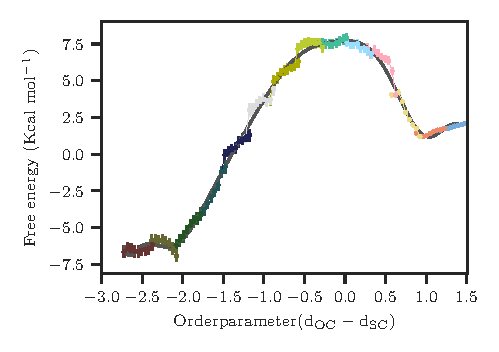
\includegraphics[scale=1.0]{figures/mat2a-fenergy.pdf}
\caption{The free energy as a function of the order 
parameter for the reaction catalyzed
by the human MAT2A enzyme. The activation barrier is 
calculated to be $16\;\text{Kcal mol}^{-1}$. The solid colored disks represent the free energies 
calculated within the individual windows which is adjusted to make the free energy as a function 
of the order parameter a continuous function.}
\label{fig:mat2a-fenergy}
\end{figure}
The free energy profile from our TPS based calculations is shown in 
Fig. \ref{fig:mat2a-fenergy}\DIFdelbegin \DIFdel{where the }\DIFdelend \DIFaddbegin \DIFadd{. It includes standard deviations calculated 
using the bootstrapping method for the populations of configurations 
sampled within each window. \mbox{%DIFAUXCMD
\cite{Hub10JChemTheoryComput6p3713}
}\hspace{0pt}%DIFAUXCMD
The calculated free energy }\DIFaddend barrier is $16\;\text{Kcal mol}^{-1}$.
\DIFdelbegin \DIFdel{This }\DIFdelend \DIFaddbegin \DIFadd{which }\DIFaddend is in excellent agreement with the experimental result.  
%------------------------------------------------------------------------------ 
\subsection{$pv$ADA}
%------------------------------------------------------------------------------ 
The equilibrated structure for the ADA enzyme complexed with adenosine, 
OH$^{-}$ anion and Zn$^{2+}$ cation is shown in Fig. \ref{fig:ada-equil}.
The Zn$^{2+}$ cation interacts with the His42, His44 and His226 residues
and stabilizes the OH$^{-}$ anion in the pocket. The N1 atom on the adensoyl 
molecule hydrogen bonds with the carboxylic acid hydrogen atom of the Glu229 
residue.  
\begin{figure}[ht!]
\centering
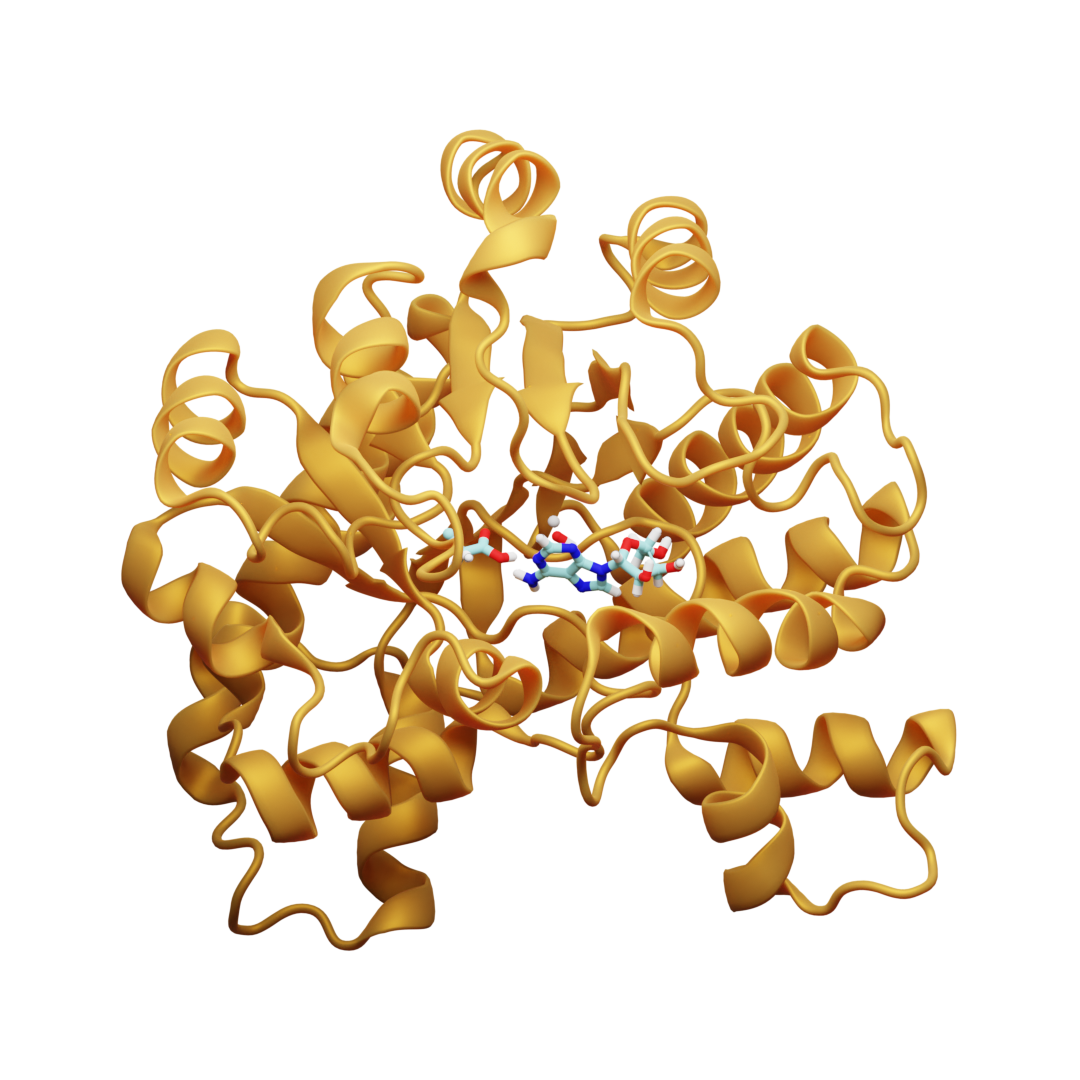
\includegraphics[scale=0.2]{./figures/ada-equil.png}
\caption{Equilibrated structure of $pv$ADA enzyme complexed with adenosine, 
OH$^{-}$ anion and Zn$^{2+}$.}
\label{fig:ada-equil}
\end{figure}
The bond forming (d$_{\text{OC}}$) and bond breaking (d$_{\text{NC}}$) distances 
for a reactive trajectory from the TPS ensemble is depicted 
in Fig. \ref{fig:ada-reactive-traj}.
\begin{figure}[ht!]
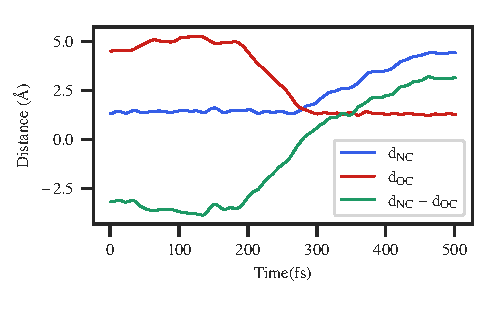
\includegraphics[scale=1.0]{figures/ada-diff60.pdf}
\caption{Bond breaking ($\mathrm{d}_{\mathrm{NC}}$), bond forming 
($\mathrm{d}_{\mathrm{OC}}$) distances for a typical 
reactive trajectory for the reaction catalyzed by the $pv$ADA enzyme.}
\label{fig:ada-reactive-traj}
\end{figure}
The deamination is an aromatic nucleophilic substitution reaction 
where an intermediate Meisenheimer complex like structure is formed 
at the transition state as shown in Fig. \ref{fig:ada-trans}. 
The approaching O atom of the OH$^{-}$ anion is at a distance of $1.49$ {\AA}
from the C6 atom whereas the N atom of the amine leaving group is at $1.62$ {\AA}
from the C6 atom.
The N$1-$H bond distance is $1.1\;${\AA} 
suggesting that the proton transfer from the Glu229 residue is almost complete.
\begin{figure}
\centering
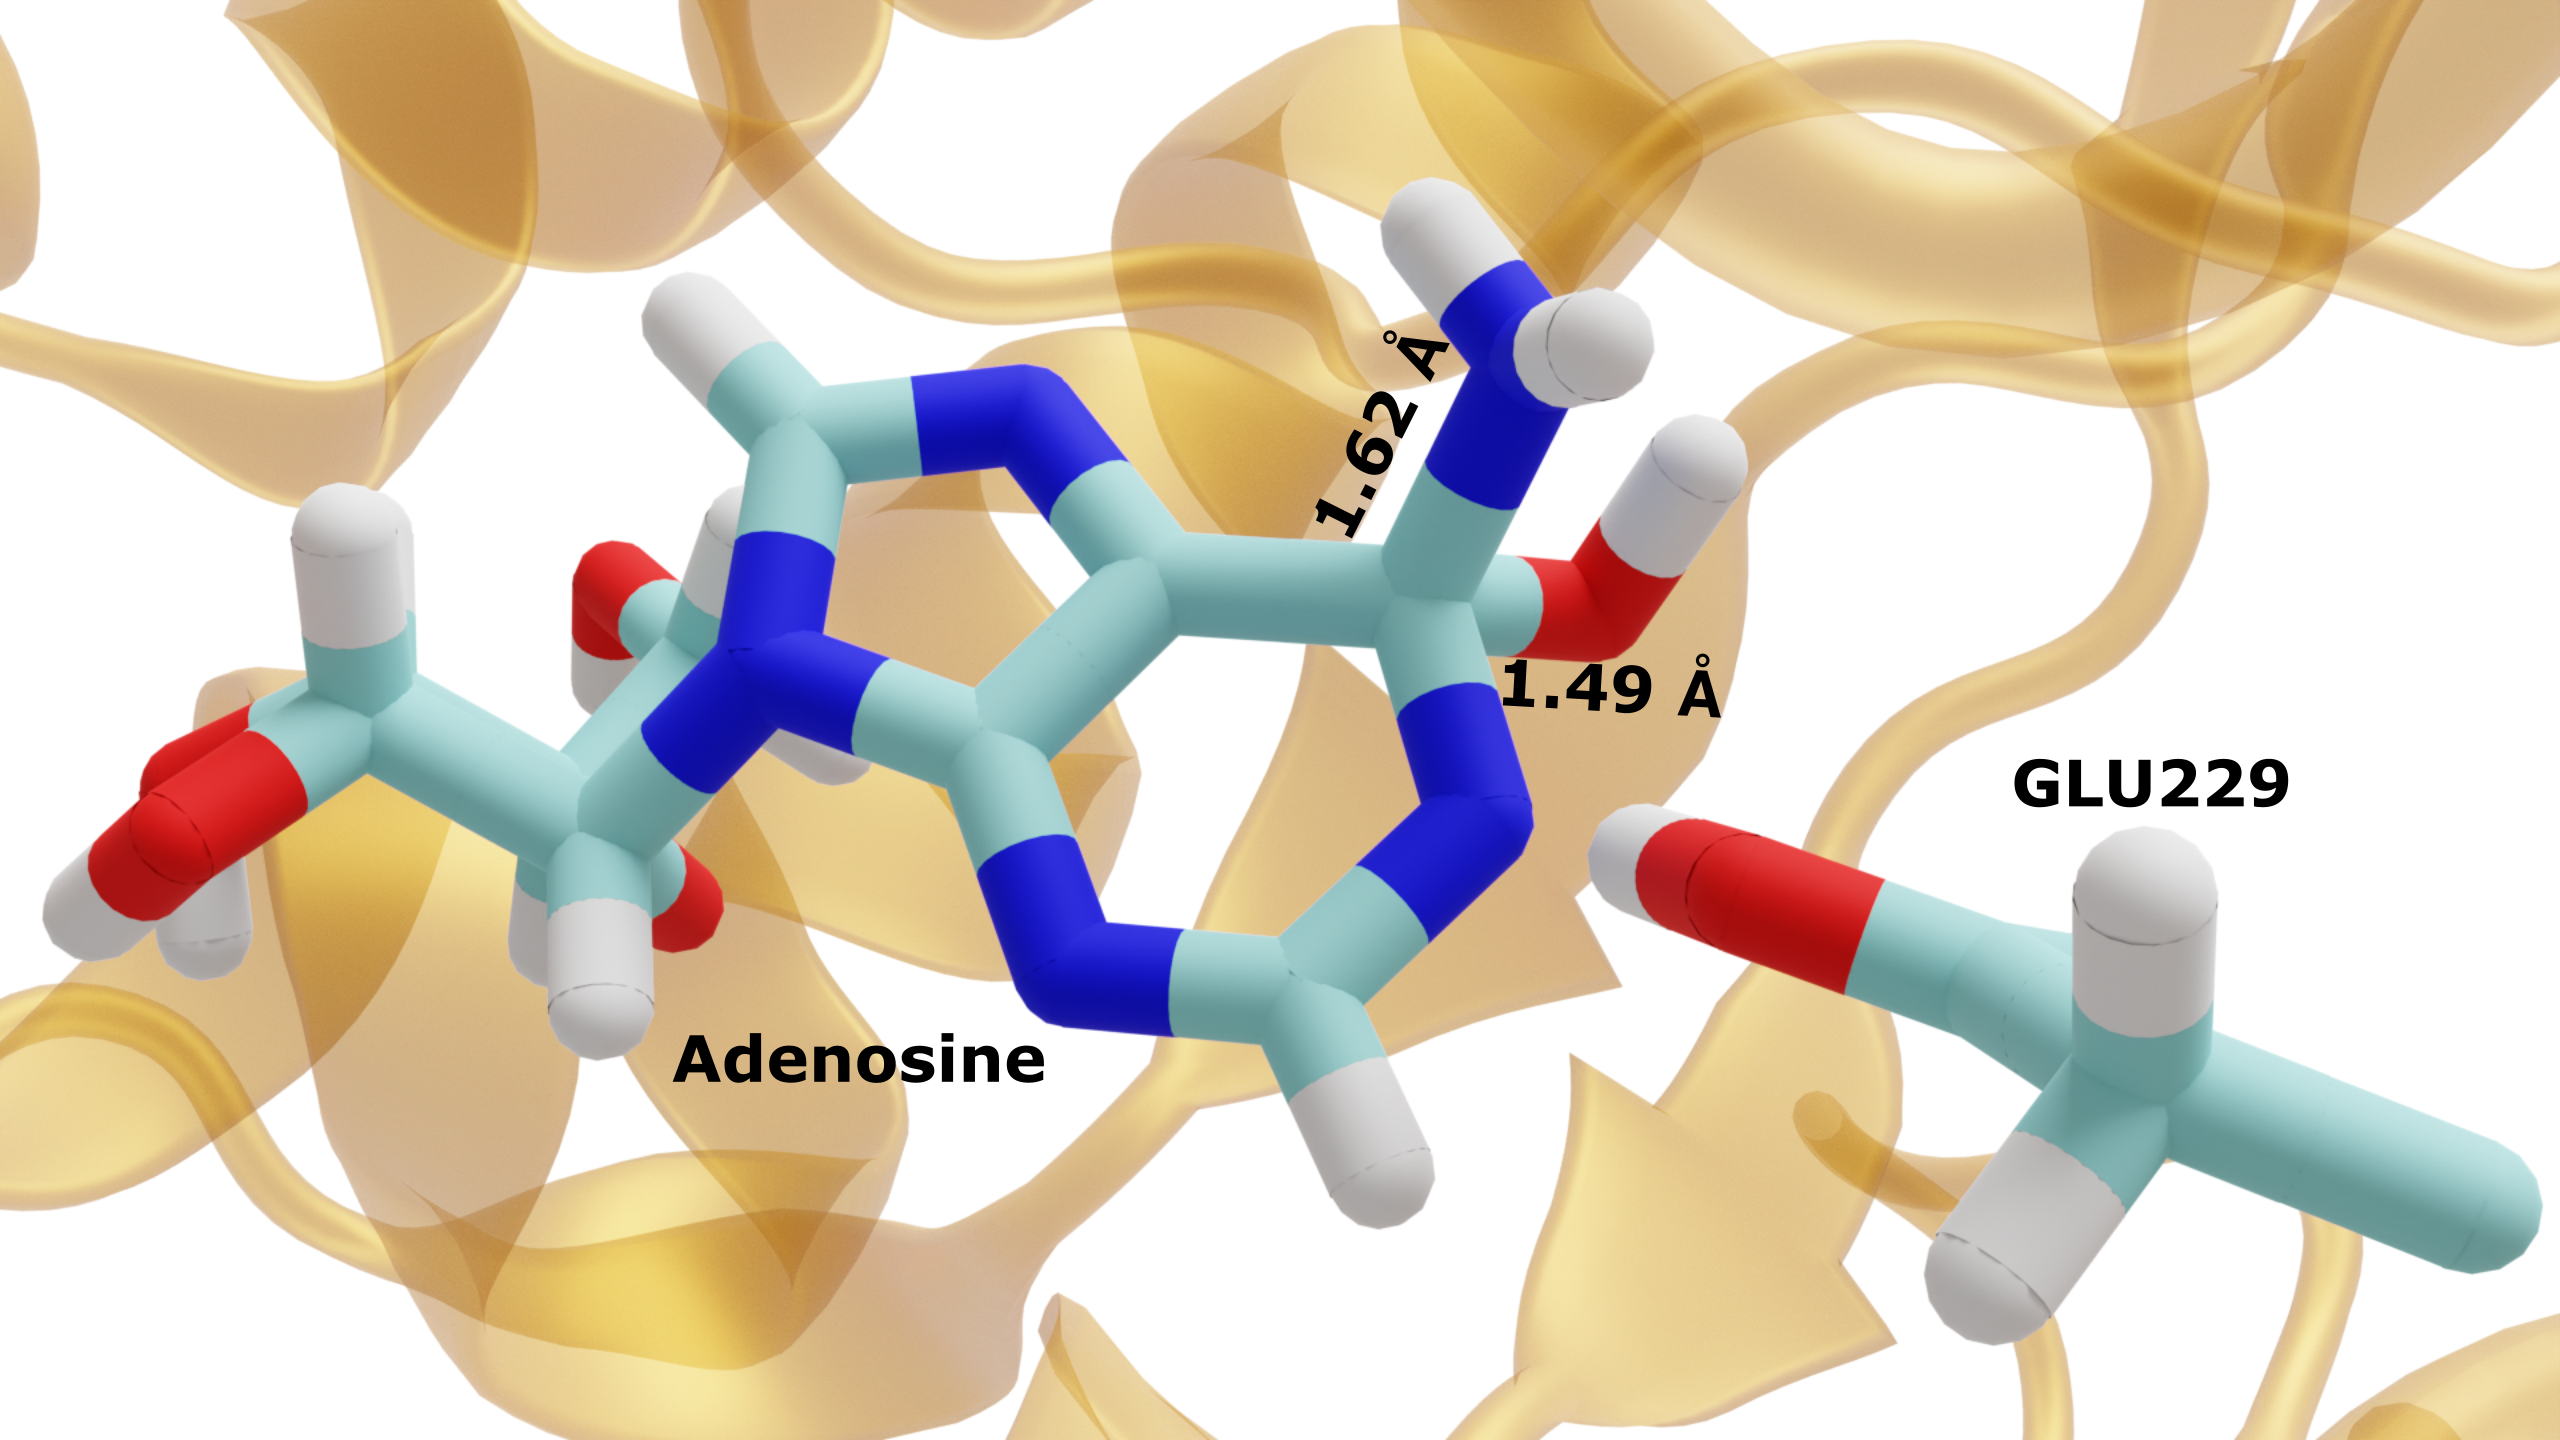
\includegraphics[scale=0.12]{figures/new-ada-trans.png}
\caption{The transition state structure of the reaction catalyzed by the ADA enzyme.
The formation of the Meisenheimer complex like structure with 
d$_{\text{NC}}=1.62$ {\AA} and d$_{\text{OC}}=1.49$ {\AA} is observed.}
\label{fig:ada-trans}
\end{figure}
These observations are consistent with the 
experimental KIE studies from Luo et al. \cite{Luo07JAmChemSoc129p8008}
who predict the transition state structure for the deamination reaction 
catalyzed by the plasmodium falciparum ADA ($pf$ADA) enzyme which shares
$72\%$ identity with the $pv$ADA enzyme that we analyze here. The next
step in the reaction is the proton transfer from the OH$^{-}$ ion to the 
amine leaving group resulting in the formation of inosine and ammonia.   
%At the transition state, experimental findings 
%suggest that the dissociation of the C6$-$N6 bond as well as the protonation of the N1 
%atom are almost complete. \cite{Luo07JAmChemSoc129p8008}
The free energy profile that we calculated is shown in Fig. \ref{fig:ada-fenergy}.  
\begin{figure}[h!]
\centering
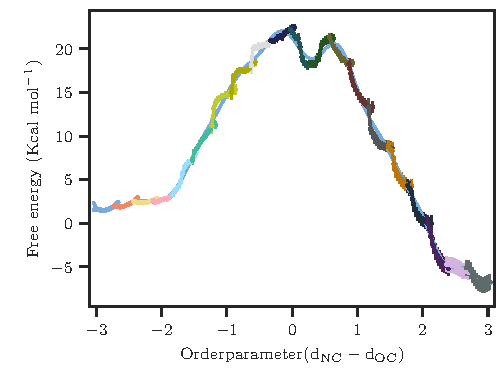
\includegraphics[scale=1.0]{figures/ada-fenergy.pdf}
\caption{The free energy as a function of the reaction 
parameter for the ADA catalyzed reaction. The activation barrier is calculated as 
$21\;\text{Kcal}\;\text{mol}^{-1}$. The solid colored disks represent the free energies 
calculated within the individual windows which is adjusted to make the free energy as a function 
of the order parameter a continuous function.}
\label{fig:ada-fenergy}
\end{figure}
The free energy \DIFaddbegin \DIFadd{profile along with standard deviations calculated 
using the bootstrapping method for the populations of configurations 
sampled within each window \mbox{%DIFAUXCMD
\cite{Hub10JChemTheoryComput6p3713} }\hspace{0pt}%DIFAUXCMD
is 
depicted in Fig. \ref{fig:ada-fenergy}.
The free energy }\DIFaddend barrier is calculated to be $21\;\text{Kcal}\;\text{mol}^{-1}$
and the overall shape of the function is very similar to that hypothesized 
by Luo et al. \cite{Luo07JAmChemSoc129p8008}
%------------------------------------------------------------------------------ 
\section{Conclusions}
%------------------------------------------------------------------------------ 
In this study, we presented an application of the TPS method for the calculation 
of free energy profiles of enzymatic reactions. The order parameter along which the 
free energy profile is to be obtained is partitioned into windows as is done in 
umbrella sampling, but instead of using bias potentials to sample the configurations
within the windows the shooting algorithm is used to
obtain an ensemble of trajectories according to the Monte Carlo algorithm. A 
trajectory is accepted if it visits the window at least in one of the time steps. 
Using this ensemble of trajectories the unbiased equilibrium probability distribution 
function of the order parameter of the reaction within each window is obtained.
Furthermore the free energy as a function of the order parameter is computed within 
each of the windows and the entire profile is obtained by shifting the free energies
such that the function is continuous at the boundaries.   

The MAT2A enzymatic reaction was analyzed in detail to elucidate the transition state,
reaction coordinate and the free energy profile. The reaction proceeds through a 
S$_\text{N}$2 mechanism, the d$_{\text{OC}}$ and d$_{\text{SC}}$ are $2.09$ {\AA}
and $2.31$ {\AA}, respectively. The reaction coordinate is determined to involve  
the Gln113, Ser114, Arg249 and Arg264 residues. 
The free energy barrier for this reaction was calculated to be 
$16\;\text{Kcal}\;\text{mol}^{-1}$ which is in good agreement 
with the experimentally measured activation energy of $17.27\;\pm\;1.5\;\text{Kcal mol}^{-1}$. 
Furthermore the reaction catalyzed by the $pv$ADA enzyme is analyzed in detail to obtain the  
transition state and calculate the free energy profile.
The transition state has a Meisenheimer complex like structure with the 
d$_\text{NC}$ and d$_\text{OC}$ being $1.62$ {\AA} and $1.49$ {\AA}, respectively.
The free energy barrier for this reaction for found to be $21\;\text{Kcal}\;\text{mol}^{-1}$
with a double well shape similar to that measured from experiments. 
These results show that free energy simulations based on unbiased transition 
path sampling computations can result in accurate and computationally
efficient predictions of both free energy profiles and mechanisms.
\DIFaddbegin \DIFadd{Free energy calculations within the TPS shooting algorithm do not employ any 
bias forces constraining the trajectories within a defined window. 
We observe that in regions where the free energy curve has a large 
slope the trajectories tend to majorly sample configurations that are 
outside the window with acceptance percentages $\leq 10$. While this improves
the decorrelation time of the sampled trajectories, techniques within 
TPS to enhance the sampling in these regions will be necessary for its
widespread applications to complex biomolecular systems.  
}\DIFaddend %%%%%%%%%%%%%%%%%%%%%%%%%%%%%%%%%%%%%%%%%%%%%%%%%%%%%%%%%%%%%%%%%%%%%
%% The "Acknowledgement" section can be given in all manuscript
%% classes.  This should be given within the "acknowledgement"
%% environment, which will make the correct section or running title.
%%%%%%%%%%%%%%%%%%%%%%%%%%%%%%%%%%%%%%%%%%%%%%%%%%%%%%%%%%%%%%%%%%%%%
\begin{acknowledgement}
SGB acknowledges funding from the NIH through grant number GM127594.
\end{acknowledgement}

%%%%%%%%%%%%%%%%%%%%%%%%%%%%%%%%%%%%%%%%%%%%%%%%%%%%%%%%%%%%%%%%%%%%%
%% The same is true for Supporting Information, which should use the
%% suppinfo environment.
%%%%%%%%%%%%%%%%%%%%%%%%%%%%%%%%%%%%%%%%%%%%%%%%%%%%%%%%%%%%%%%%%%%%%
%DIF < \begin{suppinfo}
\DIFaddbegin \begin{suppinfo}
\DIFadd{The supporting information is available free of charge at
}\DIFaddend 



%DIF < \end{suppinfo}
\DIFaddbegin \end{suppinfo}
\DIFaddend 

%%%%%%%%%%%%%%%%%%%%%%%%%%%%%%%%%%%%%%%%%%%%%%%%%%%%%%%%%%%%%%%%%%%%%
%% The appropriate \bibliography command should be placed here.
%% Notice that the class file automatically sets \bibliographystyle
%% and also names the section correctly.
%%%%%%%%%%%%%%%%%%%%%%%%%%%%%%%%%%%%%%%%%%%%%%%%%%%%%%%%%%%%%%%%%%%%%
\bibliography{manuscript}

\end{document}
